% Arquitectura del Proyecto: Terraform AWS Production Stack
\documentclass{article}
\usepackage{tikz}
\usetikzlibrary{shapes, arrows, positioning}
\begin{document}

\section*{Arquitectura General}

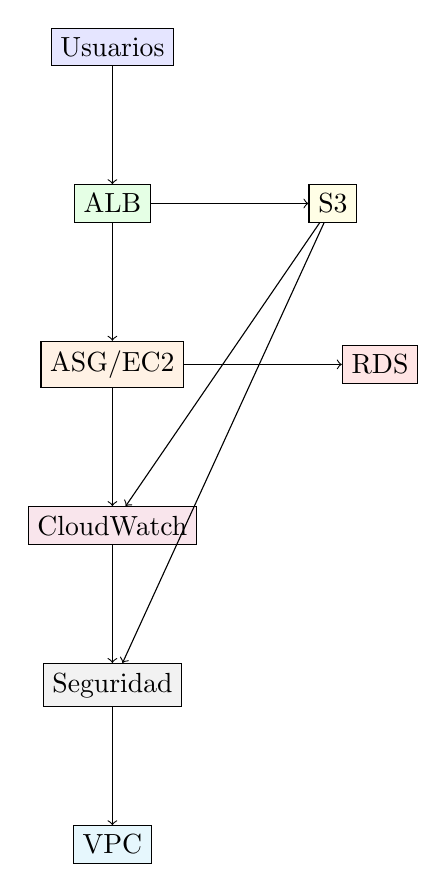
\begin{tikzpicture}[node distance=1.5cm, auto]
  % Nodes
  \node [rectangle, draw, fill=blue!10] (users) {Usuarios};
  \node [rectangle, draw, fill=green!10, below=of users] (alb) {ALB};
  \node [rectangle, draw, fill=yellow!10, right=2cm of alb] (s3) {S3};
  \node [rectangle, draw, fill=orange!10, below=of alb] (asg) {ASG/EC2};
  \node [rectangle, draw, fill=red!10, right=2cm of asg] (rds) {RDS};
  \node [rectangle, draw, fill=purple!10, below=of asg] (cloudwatch) {CloudWatch};
  \node [rectangle, draw, fill=gray!10, below=of cloudwatch] (security) {Seguridad};
  \node [rectangle, draw, fill=cyan!10, below=of security] (vpc) {VPC};

  % Edges
  \draw [->] (users) -- (alb);
  \draw [->] (alb) -- (asg);
  \draw [->] (alb) -- (s3);
  \draw [->] (asg) -- (rds);
  \draw [->] (asg) -- (cloudwatch);
  \draw [->] (cloudwatch) -- (security);
  \draw [->] (security) -- (vpc);

  % S3 connections
  \draw [->] (s3) -- (cloudwatch);
  \draw [->] (s3) -- (security);
\end{tikzpicture}

\begin{itemize}
  \item El estado de Terraform se almacena en S3 y se bloquea con DynamoDB.
  \item Los módulos permiten reutilización y orden.
  \end{itemize}

  \vspace{1cm}
  \noindent
  	extbf{Los entornos dev/prod tienen configuraciones independientes.}
\end{itemize}

\end{document}
